\documentclass[border=2pt]{standalone}
\usepackage[T1]{fontenc}
\usepackage{mathptmx}
\usepackage{tikz}
\usetikzlibrary{positioning,arrows.meta,fit,backgrounds,calc}
\definecolor{inkA}{HTML}{0B0B0B}
\definecolor{ink2}{HTML}{52514E}
\definecolor{cBlue}{HTML}{2A78D6}
\definecolor{cOrange}{HTML}{EB6834}
\definecolor{cAqua}{HTML}{1BAF7A}
\definecolor{fillA}{HTML}{FCE6DC}
\definecolor{fillB}{HTML}{DDF3EA}
\definecolor{fillC}{HTML}{DDEAF9}
\definecolor{panel}{HTML}{F6F6F4}
\tikzset{
  box/.style={draw=ink2,line width=0.4pt,rounded corners=1.5pt,align=center,
              font=\scriptsize,inner sep=2pt,minimum height=5.2mm,fill=white},
  arr/.style={-{Stealth[length=1.6mm]},line width=0.45pt,draw=ink2},
  ttl/.style={font=\footnotesize\bfseries,anchor=west,text=inkA},
  note/.style={font=\tiny,text=ink2,align=center},
}
\begin{document}
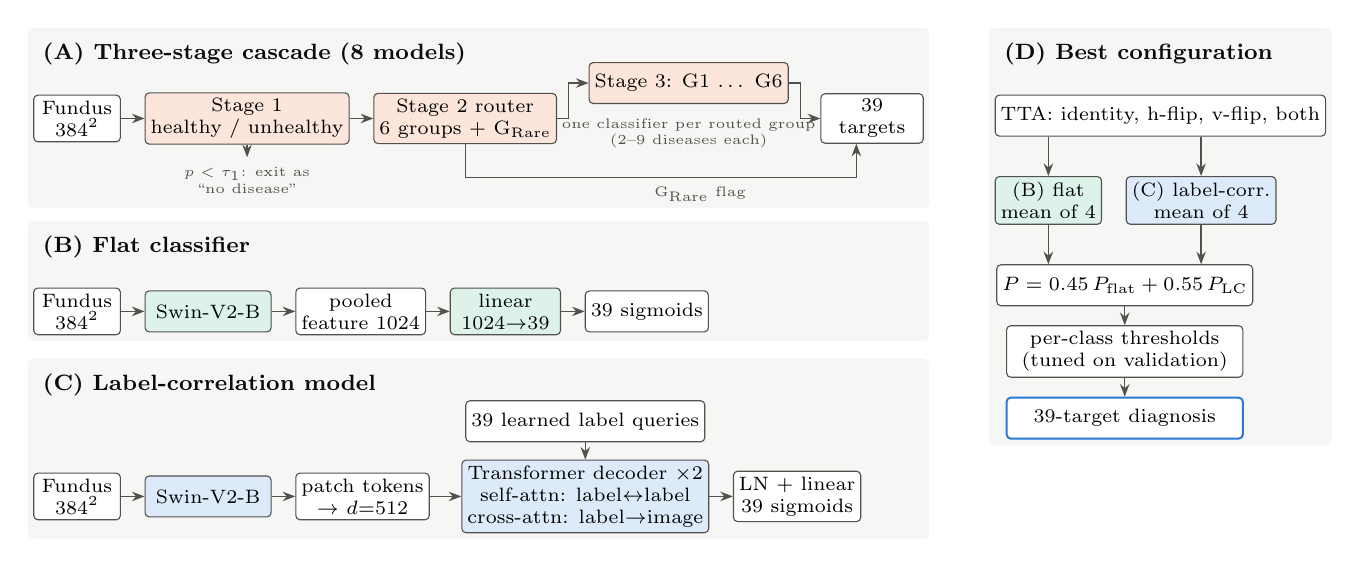
\begin{tikzpicture}[node distance=2.2mm and 3.0mm]
%% ---------------- (A) cascade ----------------
\node[ttl] (tA) at (0,0) {(A) Three-stage cascade (8 models)};
\node[box,below=2.5mm of tA.south west,anchor=north west,minimum width=11mm] (inA) {Fundus\\384$^2$};
\node[box,right=of inA,fill=fillA,minimum width=17mm] (s1) {Stage 1\\healthy / unhealthy};
\node[box,right=of s1,fill=fillA,minimum width=19mm] (s2) {Stage 2 router\\6 groups + G\textsubscript{Rare}};
\node[box,right=4mm of s2,fill=fillA,minimum width=19mm,yshift=4.5mm] (s3a) {Stage 3: G1 \dots\ G6};
\node[note,below=0.6mm of s3a] (s3n) {one classifier per routed group\\(2--9 diseases each)};
\node[box,right=4mm of s3a,yshift=-4.5mm,minimum width=13mm] (outA) {39\\targets};
\node[note,below=1.6mm of s1] (h) {$p<\tau_1$: exit as\\``no disease''};
\draw[arr] (inA) -- (s1); \draw[arr] (s1) -- (s2);
\draw[arr] (s2.east) -- ++(1.5mm,0) |- (s3a.west);
\draw[arr] (s3a.east) -- ++(1.5mm,0) |- (outA.west);
\draw[arr] (s2.south) |- ++(10mm,-4.2mm) -| ([xshift=-2mm]outA.south) node[note,pos=0.25,below]{G\textsubscript{Rare} flag};
\draw[arr,densely dashed] (s1.south) -- (h.north);

%% ---------------- (B) flat ----------------
\node[ttl] (tB) at (0,-2.45) {(B) Flat classifier};
\node[box,below=2.5mm of tB.south west,anchor=north west,minimum width=11mm] (inB) {Fundus\\384$^2$};
\node[box,right=of inB,fill=fillB,minimum width=16mm] (bbB) {Swin-V2-B};
\node[box,right=of bbB,minimum width=15mm] (poolB) {pooled\\feature 1024};
\node[box,right=of poolB,fill=fillB,minimum width=14mm] (linB) {linear\\1024$\to$39};
\node[box,right=of linB,minimum width=13mm] (outB) {39 sigmoids};
\draw[arr] (inB)--(bbB); \draw[arr] (bbB)--(poolB); \draw[arr] (poolB)--(linB); \draw[arr] (linB)--(outB);

%% ---------------- (C) label correlation ----------------
\node[ttl] (tC) at (0,-4.2) {(C) Label-correlation model};
\node[box,below=8.5mm of tC.south west,anchor=north west,minimum width=11mm] (inC) {Fundus\\384$^2$};
\node[box,right=of inC,fill=fillC,minimum width=16mm] (bbC) {Swin-V2-B};
\node[box,right=of bbC,minimum width=15mm] (tok) {patch tokens\\$\to$ $d{=}512$};
\node[box,right=4mm of tok,fill=fillC,minimum width=26mm,minimum height=9mm] (dec)
     {Transformer decoder $\times 2$\\self-attn: label$\leftrightarrow$label\\cross-attn: label$\to$image};
\node[box,above=2.2mm of dec,minimum width=26mm] (q) {39 learned label queries};
\node[box,right=of dec,minimum width=13mm] (outC) {LN + linear\\39 sigmoids};
\draw[arr] (inC)--(bbC); \draw[arr] (bbC)--(tok); \draw[arr] (tok)--(dec);
\draw[arr] (q)--(dec); \draw[arr] (dec)--(outC);

%% ---------------- (D) best configuration ----------------
\coordinate (Dx) at ($(outA.east)+(9mm,0)$);
\node[ttl] (tD) at (Dx|-tA) {(D) Best configuration};
\node[box,below=2.5mm of tD.south west,anchor=north west,minimum width=30mm] (tta)
     {TTA: identity, h-flip, v-flip, both};
\node[box,below=5mm of tta.south west,anchor=north west,fill=fillB,minimum width=13.5mm] (mB) {(B) flat\\mean of 4};
\node[box,right=3mm of mB,fill=fillC,minimum width=13.5mm] (mC) {(C) label-corr.\\mean of 4};
\coordinate (mid) at ($(mB.south)!0.5!(mC.south)$);
\node[box,below=5mm of mid,minimum width=30mm] (blend) {$P = 0.45\,P_{\mathrm{flat}} + 0.55\,P_{\mathrm{LC}}$};
\node[box,below=2.4mm of blend,minimum width=30mm] (thr) {per-class thresholds\\(tuned on validation)};
\node[box,below=2.4mm of thr,minimum width=30mm,draw=cBlue,line width=0.7pt] (outD) {39-target diagnosis};
\draw[arr] (tta.south-|mB) -- (mB); \draw[arr] (tta.south-|mC) -- (mC);
\draw[arr] (mB.south) -- (mB.south|-blend.north); \draw[arr] (mC.south) -- (mC.south|-blend.north);
\draw[arr] (blend)--(thr); \draw[arr] (thr)--(outD);

\coordinate (rB) at (outA.east|-outB);
\coordinate (rC) at (outA.east|-dec);
\begin{scope}[on background layer]
  \node[fill=panel,rounded corners=2pt,fit=(tA)(inA)(outA)(h)(s3n),inner sep=2pt] {};
  \node[fill=panel,rounded corners=2pt,fit=(tB)(inB)(outB)(rB),inner sep=2pt] {};
  \node[fill=panel,rounded corners=2pt,fit=(tC)(inC)(outC)(q)(dec)(rC),inner sep=2pt] {};
  \node[fill=panel,rounded corners=2pt,fit=(tD)(tta)(outD)(mC),inner sep=2pt] {};
\end{scope}
\end{tikzpicture}
\end{document}
